\documentclass[ignoreonframetext,unicode]{beamer}

\usepackage[utf8]{inputenc}
\usepackage[T1]{fontenc}
\usepackage[english,russian]{babel}
\usepackage{amsmath}
\usepackage{amsfonts}
\usepackage{amssymb}
\usepackage{graphicx,pgf}
\usepackage{multimedia}
%\usepackage{hyperref}
%\usepackage{enumitem}
\graphicspath{{./style/}{./pictures/}}

%\usetheme{Rochester}  %тема без навигации
%\usetheme{Montpellier} %тема с навигацией в виде дерева
%\usetheme{Berkeley} %тема с оглавлением на полях
%\usetheme{Berlin} %тема с навигацией в виде мини-слайдов

\usetheme{Warsaw} %тема с таблицей разделов и подразделов

\useinnertheme{circles}   %внутренняя тема
%\useoutertheme{smoothbars}   %внешняя тема
\usecolortheme{seahorse}    %цветовая схема
%\usefonttheme{serif}    %шрифты

\setbeameroption{hide notes}

%номера слайдов
\newcommand*\oldmacro{}%
\let\oldmacro\insertshorttitle%
\renewcommand*\insertshorttitle{%
	\oldmacro\hfill%
	\insertframenumber\,/\,\inserttotalframenumber}
\RequirePackage{caption}
\DeclareCaptionLabelSeparator{defffis}{ }
\captionsetup{justification=centering,labelsep=defffis}

\title{Задача коммивояжера}
\subtitle{Метод полного перебора и алгоритм имитации отжига}
\author{А.И.~Колесников \and В.Г.~Пиневич}
\institute[]{МГТУ им. Н.Э.~Баумана}
\date{\today}
\titlegraphic{
\includegraphics[width=2cm]{logo.png}}


\begin{document}
	
\begin{frame}[plain]
		\maketitle
\end{frame}

%________________________________________________________________________________
\begin{frame}{Формулировка задачи}

	\begin{columns}
		\begin{column}{0.65\textwidth}
		\begin{itemize}
			
		\item Каждое ребро является характеризуется весом – положительным числом – стоимостью движения по нему.
		
		\item Найдем такой обход графа, который будет включать ровно один раз каждую его вершину. Такой обход называется гамильтоновым циклом.
			
		\item Задача коммивояжера заключается в том, чтобы найти гамильтоновый цикл минимальной стоимости.
		\end{itemize}	
		\end{column}
		\begin{column}{0.4\textwidth}
		\begin{figure}[!h]
			\begin{center}
				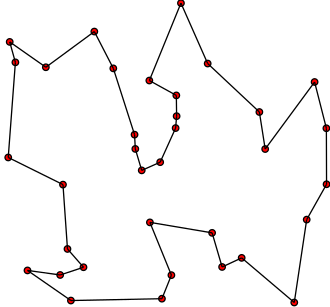
\includegraphics[scale=0.35]{SMP_pic}
			\end{center}
		\end{figure}
	
		\begin{figure}[!h]
			\begin{center}
				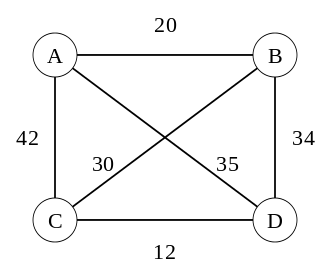
\includegraphics[scale=0.35]{Weighted_graph}
			\end{center}
		\end{figure}
		\end{column}
	\end{columns}
\end{frame}

%________________________________________________________________________________
\begin{frame}{Метод полного перебора}
		\vspace{0.5cm}
		\begin{columns}
		\begin{column}{0.4\textwidth}
			\begin{figure}[!h]
				\begin{center}
					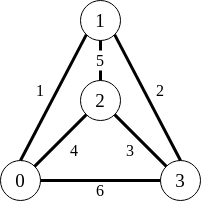
\includegraphics[scale=0.5]{Test2}
				\end{center}
			\end{figure}
		\end{column}
		\begin{column}{0.3\textwidth}
			Перестановки:
			
			\texttt{
				\begin{tabular}{ccc}
					1 & 2 & 3\\
					1 & 3 & 2\\
					2 & 1 & 3\\
					2 & 3 & 1\\
					3 & 1 & 2\\
					3 & 2 & 1\\
				\end{tabular}\\
			}
		\end{column}
		\begin{column}{0.35\textwidth}
				Потенциальные пути:
			
			\texttt{
				\begin{tabular}{ccccc}
					0 & 1 & 2 & 3 & 0\\
					0 & 1 & 3 & 2 & 0\\
					0 & 2 & 1 & 3 & 0\\
					0 & 2 & 3 & 1 & 0\\
					0 & 3 & 1 & 2 & 0\\
					0 & 3 & 2 & 1 & 0\\
				\end{tabular}\\
			}
		\end{column}
	\end{columns}
	\vspace{0.5cm}
	Из всех полученных путей выбираем путь с минимальной длиной. 
	
	Ответ : 0 1 3 2 0
\end{frame}

%________________________________________________________________________________
\begin{frame}{Алгоритм имитации отжига} 
%\vspace{2.5mm}
\begin{columns}
	\begin{column}{0.7\textwidth}
	\begin{figure}[!h]
	\begin{center}
		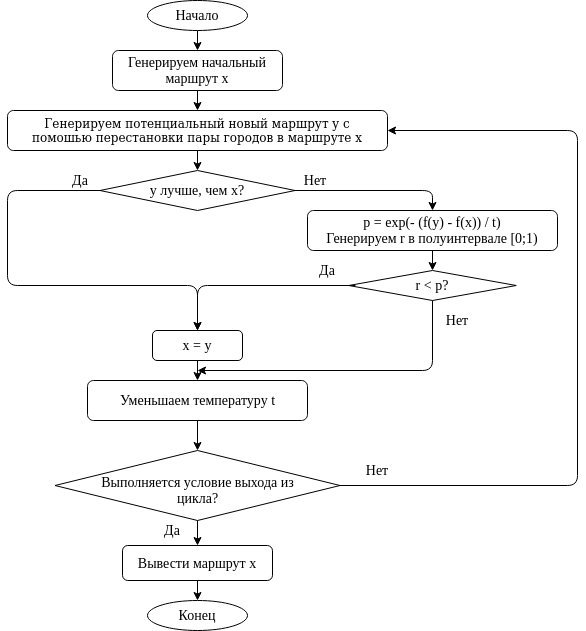
\includegraphics[scale=0.35]{Untitled_Diagram}
	\end{center}
	\end{figure}	
	\end{column}
	\begin{column}{0.5\textwidth}
		\begin{figure}[!h]
			\begin{center}
				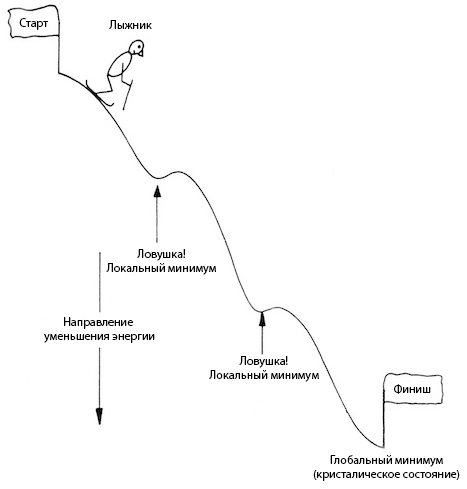
\includegraphics[scale=0.4]{ski}
			\end{center}
		\end{figure}
	\end{column}
\end{columns}	
\end{frame}

%________________________________________________________________________________
\begin{frame}{Пример 1}
	\begin{columns}
		\begin{column}{0.3\textwidth}
		\begin{block}{Исходные данные}
		\texttt{4\\
				0 1 4 6\\
				1 0 5 2\\
				4 5 0 3\\
				6 2 3 0}
		\end{block}
		\end{column}
		\begin{column}{0.3\textwidth}
			\begin{figure}[!h]
				\begin{center}
					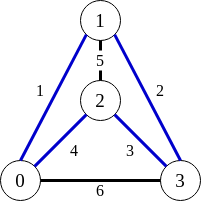
\includegraphics[scale=0.4]{Test2-1}
				\end{center}
			\end{figure}
		\end{column}
	\end{columns}	
	
\begin{table}[h]
	\begin{center}
		\small{
		\begin{tabular}{|p{0.3\linewidth}|p{0.12\linewidth}|p{0.08\linewidth}|p{0.2\linewidth}|p{0.17\linewidth}|} \hline
			%\multirow{3}*{} 
			& Маршрут & Длина пути & Относительная погрешность, \% & Затраченное время, с\\ \hline
			Метод перебора & 1 3 4 2 1 & 10 & 0,0 & 0,004 \\
			\hline
			Метод имитации отжига при {$\texttt{coolingRate}=0.1$}, $\texttt{repeatRate}=1$ & 1 3 4 2 1 & 10 & 0,0 & 0,003 \\
			\hline
		\end{tabular}\\
	}
	\end{center}
\end{table}

\end{frame}

%________________________________________________________________________________
\begin{frame}{Пример 2}
\begin{table}[h]
	\small{
	\begin{center}
		\begin{tabular}{|p{0.3\linewidth}|p{0.22\linewidth}|p{0.2\linewidth}|p{0.17\linewidth}|} \hline
			& Средняя длина полученного пути & Относительная погрешность, \% & Затраченное время, с\\ \hline
			Полный перебор                               & 0,015
			& 0   & 0,034 \\ \hline
			Алгоритм имитации отжига при $\texttt{coolingRate}=0.1$, $\texttt{repeatRate}=10$ & 0,11 & 633 & 0,005 \\ \hline
			Алгоритм имитации отжига при $\texttt{coolingRate}=~0.99$, $\texttt{repeatRate}=1$ & 0,015 & 0 & 0,002 \\ \hline
			Алгоритм имитации отжига при $\texttt{coolingRate}=0.9$, $\texttt{repeatRate}=10$ & 0,033 & 120 & 0,005 \\ \hline
		\end{tabular}
	\end{center}
}
\end{table}

\end{frame}

%________________________________________________________________________________
\begin{frame}{Пример 3}
	
\begin{table}[h]
	\small{
	\begin{center}
		\begin{tabular}{|p{0.11\linewidth}|p{0.09\linewidth}|p{0.25\linewidth}|p{0.23\linewidth}|p{0.14\linewidth}|
				p{0.2\linewidth}|} \hline
			\texttt{cooling Rate} & \texttt{repeat Rate} & Средняя длина полученного пути & Относительная погрешность, \% & Затраченное время, с\\ \hline
			0,9 & 100   & 0,042 & 151  & 0,078 \\ \hline
			0,99 & 1   & 0,018 & 5,8  & 0,003 \\ \hline
			0,99 & 10   & 0,0179 & 5,68  & 0,003 \\ \hline
			0,999 & 1   & 0,018 & 5,8  & 0,005 \\ \hline
			0,999 & 10   & 0,0177 & 4,17  & 0,020 \\ \hline
			0,999 & 100   & 0,0179 & 5,31  & 0,165 \\ \hline
			0,9999 & 10   & 0,0179 & 5,65  & 0,112 \\ \hline
			0,9999 & 100   & 0,0178 & 4,86  & 0,955 \\ \hline
		\end{tabular}
	\end{center}
}
\end{table}

\end{frame}	

\begin{frame}{Выводы}
	\begin{itemize}
		
	\item Метод перебора не может быть использован для вычислений маршрута коммивояжера для достаточно больших графов. Применение этого метода на практике не представляется возможным, поскольку его алгоритмическая сложность $o(n!)$.
	
	\item Метод имитации отжига является методом приближенного вычисления и требует подбора параметров в зависимости от входных данных, однако позволяет находить решения для более сложных задач, чем метод перебора.
	\end{itemize}
\end{frame}

\end{document}